\documentclass{article}
\usepackage{amsmath}
\usepackage{enumitem}
\usepackage{amssymb}
\usepackage{booktabs}
\usepackage{tikz}
\usetikzlibrary{automata,positioning}

% Match the list format in Sipser.
\setlist[enumerate,1]{label=\textbf{\alph*.}}

% Set the exercises number and your name.
\title{Exercises \#2}
\author{Maxwell Petersen}

% No need to change these 4 lines.
\makeatletter
\newcommand\exercise[1]{\par\vspace{4ex}\normalfont\normalsize\noindent
\textbf{\large Exercise #1}\par\nobreak\@afterindentfalse\@afterheading}
\makeatother


\begin{document}
\maketitle

\exercise{1.1}
\begin{enumerate}
\item $M_1 $:$ q_1 \newline M_2 $:$ q_1$
\item $M_1 $:$ \{q_2\} \newline M_2 $:$ \{q_1, q_4\}$
\item $M_1 $:$ q_1 \rightarrow q_2 \rightarrow q_3 \rightarrow q_1 \rightarrow q_1 \newline M_2 $:$ q_1 \rightarrow q_1 \rightarrow q_1 \rightarrow q_2 \rightarrow q_4$
\item $M_1 $: No $\newline M_2 $: Yes
\item $M_1 $: No $\newline M_2 $: Yes
\end{enumerate}

\exercise{1.2}
$M_1 = (\{q_1, q_2, q_3\}, \{$a, b$\}, \delta_1, q_1, \{q_2\})\newline$
\begin{table}[h!]
  \begin{center}
    \label{tab:table1}
    \begin{tabular}{l|c r}
       $\delta_1$   &  a  &  b \\
      \hline
      $q_1$ & $q_2$ & $q_1$\\
      $q_2$ & $q_3$ & $q_3$\\
      $q_3$ & $q_2$ & $q_1$\\
    \end{tabular}
  \end{center}
\end{table}
$M_2 = (\{q_1, q_2, q_3, q_4\}, \{$a, b$\}, \delta_2, q_1, \{q_1, q_4\})$
\begin{table}[h!]
  \begin{center}
    \begin{tabular}{l|c r}
      $\delta_2$  &  a  &  b \\
      \hline
      $q_1$ & $q_1$ & $q_2$\\
      $q_2$ & $q_3$ & $q_4$\\
      $q_3$ & $q_2$ & $q_1$\\
      $q_4$ & $q_3$ & $q_4$\\
    \end{tabular}
  \end{center}
\end{table}

\exercise{1.3}
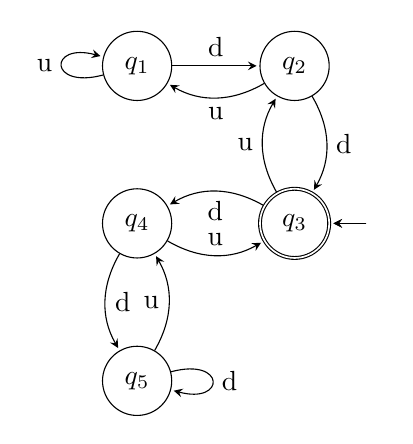
\begin{tikzpicture}[->,>=stealth,shorten >=1pt,auto ,node distance=2cm,initial text=]
  \node[state]        (q1){$q_1$};
  \node[state]        (q2) [right of=q1]  {$q_2$};
  \node[initial,state,accepting,initial right]         (q3)[below of=q2]{$q_3$};
  \node[state]	    (q4) [left of=q3]  {$q_4$};
  \node[state]	    (q5) [below of=q4] {$q_5$};

  \path[->] (q1)  edge [loop left] node {u} (q1)
             edge              node {d} (q2)
        (q2) edge [bend left]  node {u} (q1)
               edge [bend left] node {d} (q3)
        (q3) edge [bend left] node {u} (q2)
               edge [bend right]  node {d} (q4)
        (q4) edge [bend right] node {u} (q3)
               edge [bend right] node {d} (q5)
        (q5) edge [bend right]node {u} (q4)
               edge [loop right] node {d} (q5);
\end{tikzpicture}

\exercise{1.4}
\begin{enumerate}
\addtocounter{enumi}{2}
\item
$\\$
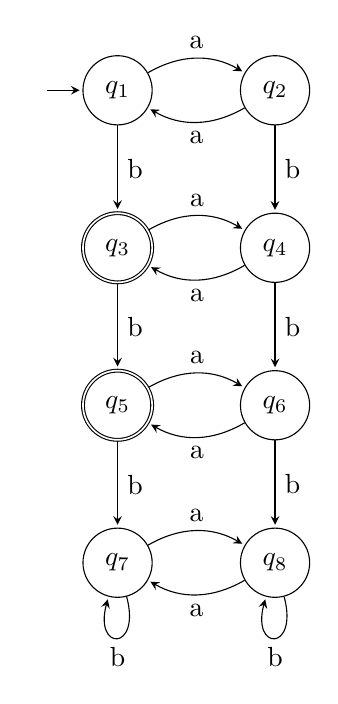
\begin{tikzpicture}[->,>=stealth,shorten >=1pt,auto,node distance=2cm,initial text=]
  \node[initial,state]        (q1){$q_1$};
  \node[state]        (q2) [right of=q1]  {$q_2$};
  \node[state,accepting]        (q3) [below of=q1]{$q_3$};
  \node[state]	    (q4) [right of=q3]  {$q_4$};
  \node[state,accepting]	    (q5) [below of=q3] {$q_5$};
  \node[state]	    (q6) [right of=q5] {$q_6$};
  \node[state]         (q7) [below of=q5] {$q_7$};
  \node[state]         (q8) [right of=q7] {$q_8$};

  \path[->] (q1)  edge  node {b} (q3)
               edge [bend left] node {a} (q2)
        (q2) edge [bend left]  node {a} (q1)
               edge node {b} (q4)
        (q3) edge [bend left] node {a} (q4)
               edge  node {b} (q5)
        (q4) edge [bend left] node {a} (q3)
               edge  node {b} (q6)
        (q5) edge [bend left]node {a} (q6)
               edge  node {b} (q7)
        (q6) edge [bend left] node {a} (q5)
               edge node {b} (q8)
        (q7) edge [bend left] node {a} (q8)
               edge [loop below] node {b} (q7)
        (q8) edge [bend left] node {a} (q7)
               edge [loop below] node {b}(q8);
\end{tikzpicture}
\cleardoublepage
$\\$
\addtocounter{enumi}{1}
$\\$
\item
$\\$
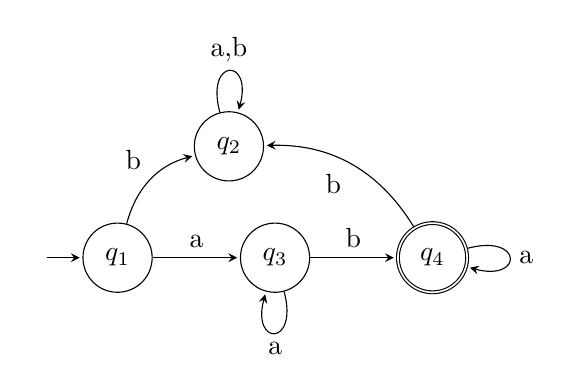
\begin{tikzpicture}[->,>=stealth,shorten >=1pt,auto ,node distance=2cm,initial text=]
  \node[initial,state]        (q1){$q_1$};
  \node[state]        (q2) [above right of=q1]  {$q_2$};
  \node[state]        (q3) [right of=q1]{$q_3$};
  \node[state,accepting]	    (q4) [right of=q3]  {$q_4$};

  \path[->] (q1)  edge node {a} (q3)
               edge [bend left]node {b} (q2)
        (q2) edge [loop above]  node {a,b} (q2)
        (q3) edge [loop below] node {a} (q3)
               edge node {b} (q4)
        (q4) edge [loop right] node {a} (q3)
               edge [bend right] node {b} (q2);
\end{tikzpicture}
\end{enumerate}

\exercise{1.5}
\begin{enumerate}
\addtocounter{enumi}{2}
\item
$\\$
$\{w | w$ contains the string $\mathsf{ab} \}\newline$
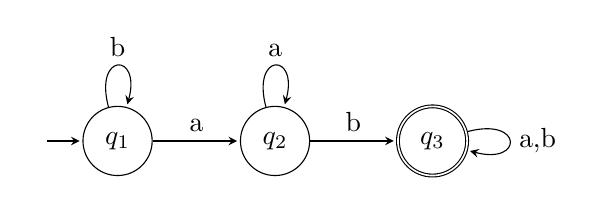
\begin{tikzpicture}[->,>=stealth,shorten >=1pt,auto ,node distance=2cm,initial text=]
  \node[initial,state]        (q1){$q_1$};
  \node[state]        (q2) [right of=q1]  {$q_2$};
  \node[state,accepting]        (q3) [right of=q2]{$q_3$};

  \path[->] (q1)  edge node {a} (q2)
               edge [loop above] node {b} (q1)
        (q2) edge [loop above] node {a} (q2)
               edge node {b} (q3)
        (q3) edge [loop right] node {a,b} (q3);
\end{tikzpicture}
$\\$
$\{w | w$ contains the string $\mathsf{ba} \}\newline$
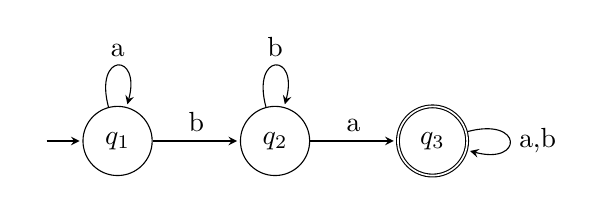
\begin{tikzpicture}[->,>=stealth,shorten >=1pt,auto ,node distance=2cm,initial text=]
  \node[initial,state]        (q1){$q_1$};
  \node[state]        (q2) [right of=q1]  {$q_2$};
  \node[state,accepting]        (q3) [right of=q2]{$q_3$};

  \path[->] (q1)  edge node {b} (q2)
               edge [loop above] node {a} (q1)
        (q2) edge [loop above] node {b} (q2)
               edge node {a} (q3)
        (q3) edge [loop right] node {a,b} (q3);
\end{tikzpicture}
$\\$
$\{w | w$ contains the string $\mathsf{ab}$ or the string $\mathsf{ba}\}\newline$
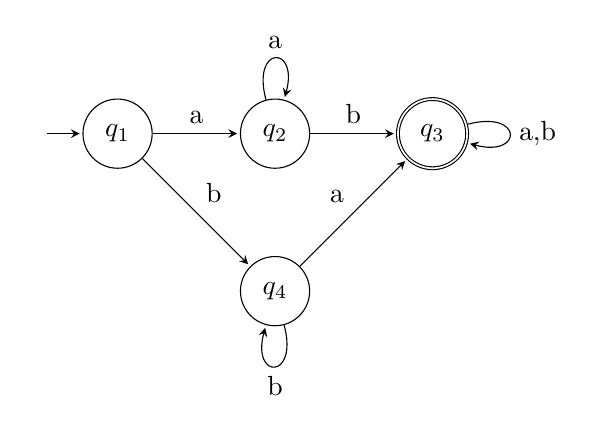
\begin{tikzpicture}[->,>=stealth,shorten >=1pt,auto ,node distance=2cm,initial text=]
  \node[initial,state]        (q1){$q_1$};
  \node[state]        (q2) [right of=q1]  {$q_2$};
  \node[state,accepting]        (q3) [right of=q2]{$q_3$};
  \node[state]        (q4) [below of=q2]{$q_4$};

  \path[->] (q1)  edge node {a} (q2)
               edge node {b} (q4)
        (q2) edge [loop above] node {a} (q2)
               edge node {b} (q3)
        (q3) edge [loop right] node {a,b} (q3)
        (q4) edge node {a}(q3)
                edge [loop below] node {b}(q4);
\end{tikzpicture}
\cleardoublepage
$\{w | w$ does not contain the string $\mathsf{ab}$ nor the string $\mathsf{ba}\}\newline$
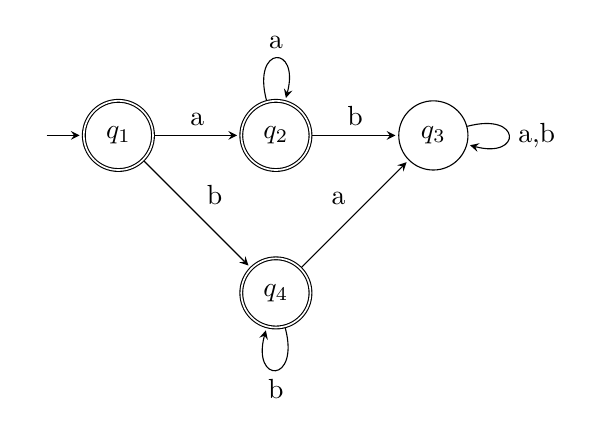
\begin{tikzpicture}[->,>=stealth,shorten >=1pt,auto ,node distance=2cm,initial text=]
  \node[initial,state,accepting]        (q1){$q_1$};
  \node[state,accepting]        (q2) [right of=q1]  {$q_2$};
  \node[state]        (q3) [right of=q2]{$q_3$};
  \node[state,accepting]        (q4) [below of=q2]{$q_4$};

  \path[->] (q1)  edge node {a} (q2)
               edge node {b} (q4)
        (q2) edge [loop above] node {a} (q2)
               edge node {b} (q3)
        (q3) edge [loop right] node {a,b} (q3)
        (q4) edge node {a}(q3)
                edge [loop below] node {b}(q4);
\end{tikzpicture}
\addtocounter{enumi}{3}
\item
$\\$
$\{w | w$ contains exactly two $\mathsf{a}$'s$\}\newline$
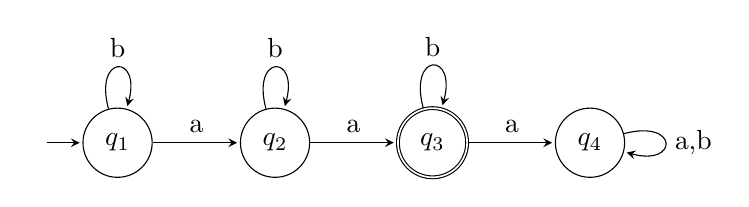
\begin{tikzpicture}[->,>=stealth,shorten >=1pt,auto ,node distance=2cm,initial text=]
  \node[initial,state]        (q1){$q_1$};
  \node[state]        (q2) [right of=q1]  {$q_2$};
  \node[state,accepting]        (q3) [right of=q2]{$q_3$};
  \node[state]        (q4) [right of=q3]{$q_4$};

  \path[->] (q1)  edge node {a} (q2)
               edge [loop above] node {b} (q1)
        (q2) edge node {a} (q3)
               edge [loop above] node {b} (q2)
        (q3) edge node {a} (q4)
               edge [loop above] node {b} (q3)
        (q4) edge [loop right] node {a,b} (q4);
\end{tikzpicture}
$\\$
$\{w | w$ doesn't contains exactly two $\mathsf{a}$'s$\}\newline$
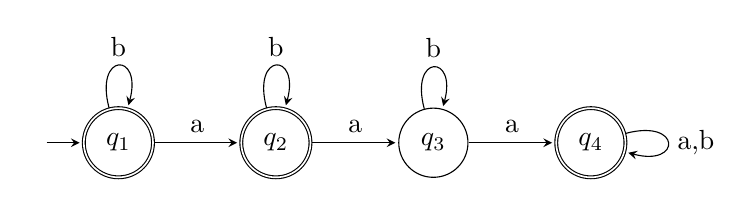
\begin{tikzpicture}[->,>=stealth,shorten >=1pt,auto ,node distance=2cm,initial text=]
  \node[initial,state,accepting]        (q1){$q_1$};
  \node[state,accepting]        (q2) [right of=q1]  {$q_2$};
  \node[state]        (q3) [right of=q2]{$q_3$};
  \node[state,accepting]        (q4) [right of=q3]{$q_4$};

  \path[->] (q1)  edge node {a} (q2)
               edge [loop above] node {b} (q1)
        (q2) edge node {a} (q3)
               edge [loop above] node {b} (q2)
        (q3) edge node {a} (q4)
               edge [loop above] node {b} (q3)
        (q4) edge [loop right] node {a,b} (q4);
\end{tikzpicture}
\end{enumerate}

\exercise{1.7}
\begin{enumerate}
\item 
$\\$
$\{w | w$ ends with $\mathsf{00}$$\}\newline$
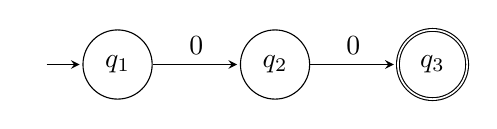
\begin{tikzpicture}[->,>=stealth,shorten >=1pt,auto ,node distance=2cm,initial text=]
  \node[initial,state]        (q1){$q_1$};
  \node[state]        (q2) [right of=q1]  {$q_2$};
  \node[state,accepting]        (q3) [right of=q2]{$q_3$};

  \path[->] (q1)  edge node {0} (q2)
        (q2) edge node {0} (q3);
\end{tikzpicture}
\item 
$\\$
$\{w | w$ contains the substring $\mathsf{0101}$$\}\newline$
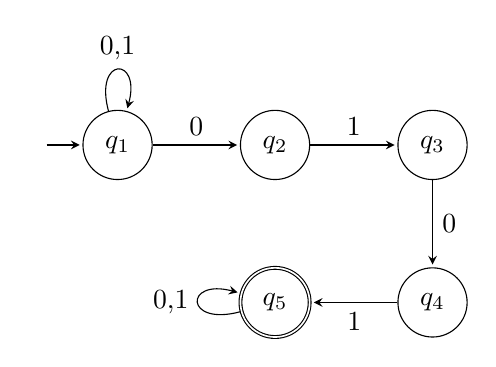
\begin{tikzpicture}[->,>=stealth,shorten >=1pt,auto ,node distance=2cm,initial text=]
  \node[initial,state]        (q1){$q_1$};
  \node[state]        (q2) [right of=q1]  {$q_2$};
  \node[state]         (q3)[right of=q2]{$q_3$};
  \node[state]	    (q4) [below of=q3]  {$q_4$};
  \node[state,accepting]	    (q5) [left of=q4] {$q_5$};

  \path[->] (q1)  edge node {0} (q2)
               edge [loop above] node {0,1} (q1)
        (q2) edge node {1} (q3)
        (q3) edge node {0} (q4)
        (q4) edge node {1} (q5)
        (q5) edge [loop left] node {0,1} (q5);
\end{tikzpicture}
\cleardoublepage
\item
$\\$
$\{w | w$ contains an even number of $\mathsf{0}$'s or exactly two $\mathsf{1}$'s$\}\newline$
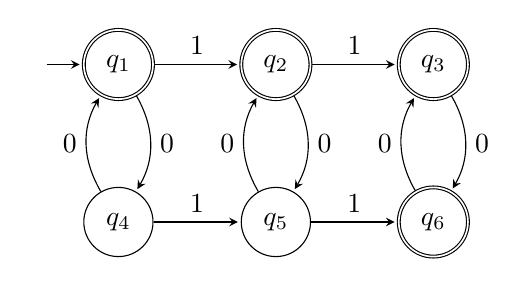
\begin{tikzpicture}[->,>=stealth,shorten >=1pt,auto ,node distance=2cm,initial text=]
  \node[initial,state,accepting]        (q1){$q_1$};
  \node[state,accepting]        (q2) [right of=q1]  {$q_2$};
  \node[state,accepting]         (q3)[right of=q2]{$q_3$};
  \node[state]	    (q4) [below of=q1]  {$q_4$};
  \node[state]	    (q5) [right of=q4] {$q_5$};
  \node[state,accepting]        (q6) [right of=q5]{$q_6$};

  \path[->] (q1)  edge [bend left] node {0} (q4)
               edge node {1} (q2)
        (q2) edge node {1} (q3)
               edge [bend left] node {0} (q5)
        (q3) edge [bend left] node {0} (q6)
        (q4) edge node {1} (q5)
               edge [bend left] node {0} (q1)
        (q5) edge node {1} (q6)
               edge [bend left] node {0} (q2)
        (q6) edge [bend left] node {0} (q3);
\end{tikzpicture}
\item 
$\\$
$\{0\}\newline$
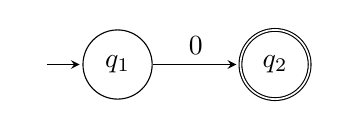
\begin{tikzpicture}[->,>=stealth,shorten >=1pt,auto ,node distance=2cm,initial text=]
  \node[initial,state]        (q1){$q_1$};
  \node[state,accepting]        (q2) [right of=q1]  {$q_2$};

  \path[->] (q1)  edge node {0} (q2);
\end{tikzpicture}
\addtocounter{enumi}{2}
\item 
$\\$
$\{\epsilon\}\newline$
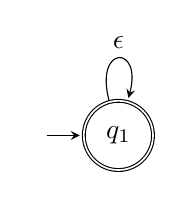
\begin{tikzpicture}[->,>=stealth,shorten >=1pt,auto ,node distance=2cm,initial text=]
  \node[initial,state,accepting]        (q1){$q_1$};

  \path[->] (q1)  edge [loop above] node {$\epsilon$} (q2);
\end{tikzpicture}
\end{enumerate}

\end{document}
